% Question:  What are the role of computer technology in society today ? Do we really need computers?


%Question: Do we really need computers?

\begin{frame}
\frametitle{Computers Technology in 1960s}
\begin{itemize}
\item Punchcards
\item invention of transistor
\item databases
\item Do simple calculations fast
\end{itemize}
\end{frame}

\begin{frame}
\frametitle{Social Media:}
\begin{itemize}
\item LinkedIn: Digitize business interactions
\item Facebook: digitize social interactions
\item Twitter: broadcast ideas
\end{itemize}
\end{frame}

\begin{frame}
\frametitle{data searching}
\begin{itemize}
\item Google:
\item Yahoo:
\item Bing:
\end{itemize}
\end{frame}



\begin{frame}
\frametitle{Hardware virtualization and making cloud work}
\begin{itemize}
\item vmware
\item symantec
\end{itemize}
\end{frame}


\begin{frame}
\frametitle{Human Computer Interaction}
\begin{itemize}
\item Apple's iPhone
\item Garmin
\item Kindle
\end{itemize}


\end{frame}


\begin{frame}
\frametitle{ Business Applications Support }
\begin{itemize}
\item salesforce
\item
\end{itemize}
\end{frame}

\begin{frame}
\frametitle{Collaboration/Management}
\begin{itemize}
\item Git:
\item Fuzebox:
\item cmake:
\end{itemize}
\end{frame}





\begin{frame}
\frametitle{Computers in practice}
\begin{itemize}
\item technology for business productivity:  salesforce, collab
\item Big Data for gmail
\item Social media and human computer interaction: facebook
\item Optimization for numerical simulations for discovery science
\end{itemize}
\end{frame}


\begin{frame}
\frametitle{What Computers can do for Science and Engineering}
\begin{itemize}
\item numerical simulations come close to doing all these things, i.e. with high ``resolution''
\item solvers can provide solutions with high ``accuracy'' (solver is ``stable'' if it generates solutions with high accuracy)
\item can accelerate science per hour
\item can accelerate engineering per hour
\end{itemize}
\end{frame}

\begin{frame}
\frametitle{Question}
How can we accelerate solving problems and make scientific discoveries in this world with the use of computer?

\end{frame}

\begin{frame}
\frametitle{Science and Engineering without computers}
\begin{itemize}
\item \small Biology, e.g. Protein Folding
\item \small Physics, e.g. Fusion
\item \small Meteorology,e.g. Simulating Tornadoes
\end{itemize}
\begin{center}
$\rightarrow$ \textbf{ Stencils}
\end{center}
\end{frame}


\begin{frame}
\frametitle{Solving Engineering Problems}
\begin{itemize}
\item \small Operations Research, e.g. UPS truck routing
\item \small Aerospace Engineering, e.g. Airflow for rocket sim
\item \small Electromagnetics, e.g. MRI scans
\end{itemize}
\begin{center}
$\rightarrow$ \textbf{ Factorizations}
\end{center}
\end{frame}


\begin{frame}
\frametitle{How HPC helps}
\begin{itemize}
\item Engineering principles,e.g. signal processing and risk analysis are needed to find the best code optimizations for stencils and factorizations
\item By optimizing codes using stencils and factorizations, runtime systems managing resources for full applications
\item by managing resources,  we can do discovery science and engineering in a cost efficient manner
\end{itemize}
\end{frame}


\begin{frame}
\frametitle{Conclusions}
\begin{itemize}
\item Engineering and Science Simulations have key computations (stencils and factorizations), we can tackle all problems at once.
\item Runtime systems allow for applying these strategies automatically to full applications
\item Cost-cutting runtimes allow for more science per hour, and more problem solving per hour
\end{itemize}
\end{frame}

%\input{elevatorSlide}

%\begin{frame}
%\frametitle{Numerical Simulations for Scientific Discovery}
%\framebox{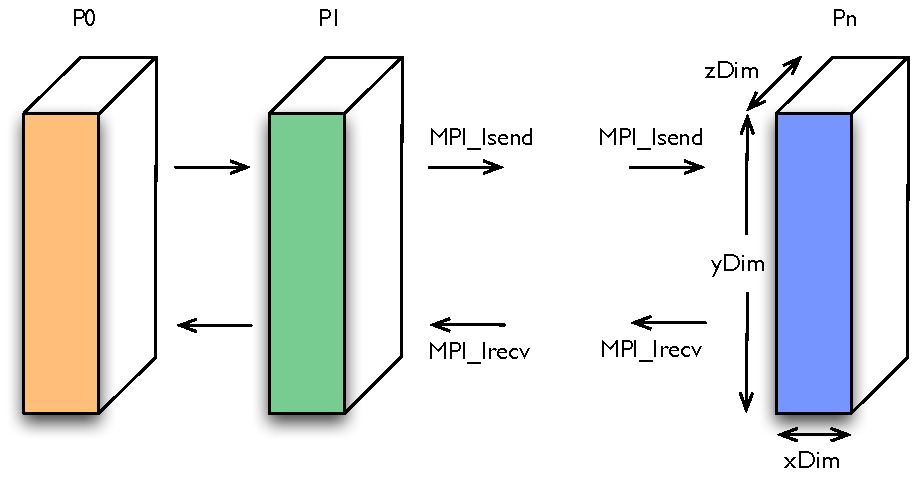
\includegraphics[width=\textwidth]{images/mpi_decomp}}
%\begin{center}
%Model bulk-synchronous Numerical Simulation
%\end{center}
%\end{frame}

%\begin{frame}
%\frametitle{Model Bulk-Synchronous MPI+OpenMP Application Code}
%\begin{center}
%\begin{figure}[ht]
%\lstinputlisting{/Users/kale2/hybridscheduling/listings/omp-static.c}
%\end{figure}
%\end{center}
%\end{frame}

\begin{frame}
\frametitle{Model Bulk-synchronous code: 1 node}
\visible<1->{\lstinputlisting{/Users/kale2/hybridscheduling/listings/mpi-bulk-synch.c}}
\begin{itemize}
\item \tiny Apps are mostly synchronous due to constraints of the application (physics simulation  must guarantee that certain values must come at certain times) .
\end{itemize}
\end{frame}


\begin{frame}
\frametitle{Model Bulk-synchronous code: 2 nodes}
\visible<1->{\lstinputlisting{/Users/kale2/hybridscheduling/listings/mpi-bulk-synch.c}}
\begin{itemize}
\item \tiny Because apps are mostly synchronous, noise delays entry into MPI call
\end{itemize}
\end{frame}


\begin{frame}
\frametitle{Model Bulk-synchronous code: 10000 nodes}
\visible<1->{\lstinputlisting{/Users/kale2/hybridscheduling/listings/mpi-bulk-synch.c}}
\end{frame}


\begin{frame}
\frametitle{Model Bulk-synchronous code: p nodes}
\visible<1->{\lstinputlisting{/Users/kale2/hybridscheduling/listings/mpi-bulk-synch.c}}
\end{frame}


\begin{frame}
\frametitle{Model Bulk-synchronous code}
\visible<1->{\lstinputlisting{/Users/kale2/hybridscheduling/listings/mpi-bulk-synch.c}}
\end{frame}

\begin{frame}[Noise Amplification Problem for Bulk-synchronous Simulations]
\frametitle{Noise Amplification Problem}
\begin{columns}
\column{0.5\textwidth}
\begin{enumerate}
\item \tiny OS noise slows down HPC codes (``disproportionately'') a lot at scale.
\item \tiny Because apps are mostly synchronous, noise delays entry into MPI call.
\item \tiny Noise likelihood insignificant on single node, but significant at very large(10000+ node) scales.
\item \tiny Hybrid apps give opportunity because they can allow for moving noise off critical path, using OpenMP model.
\end{enumerate}
\column{0.5\textwidth}
\framebox{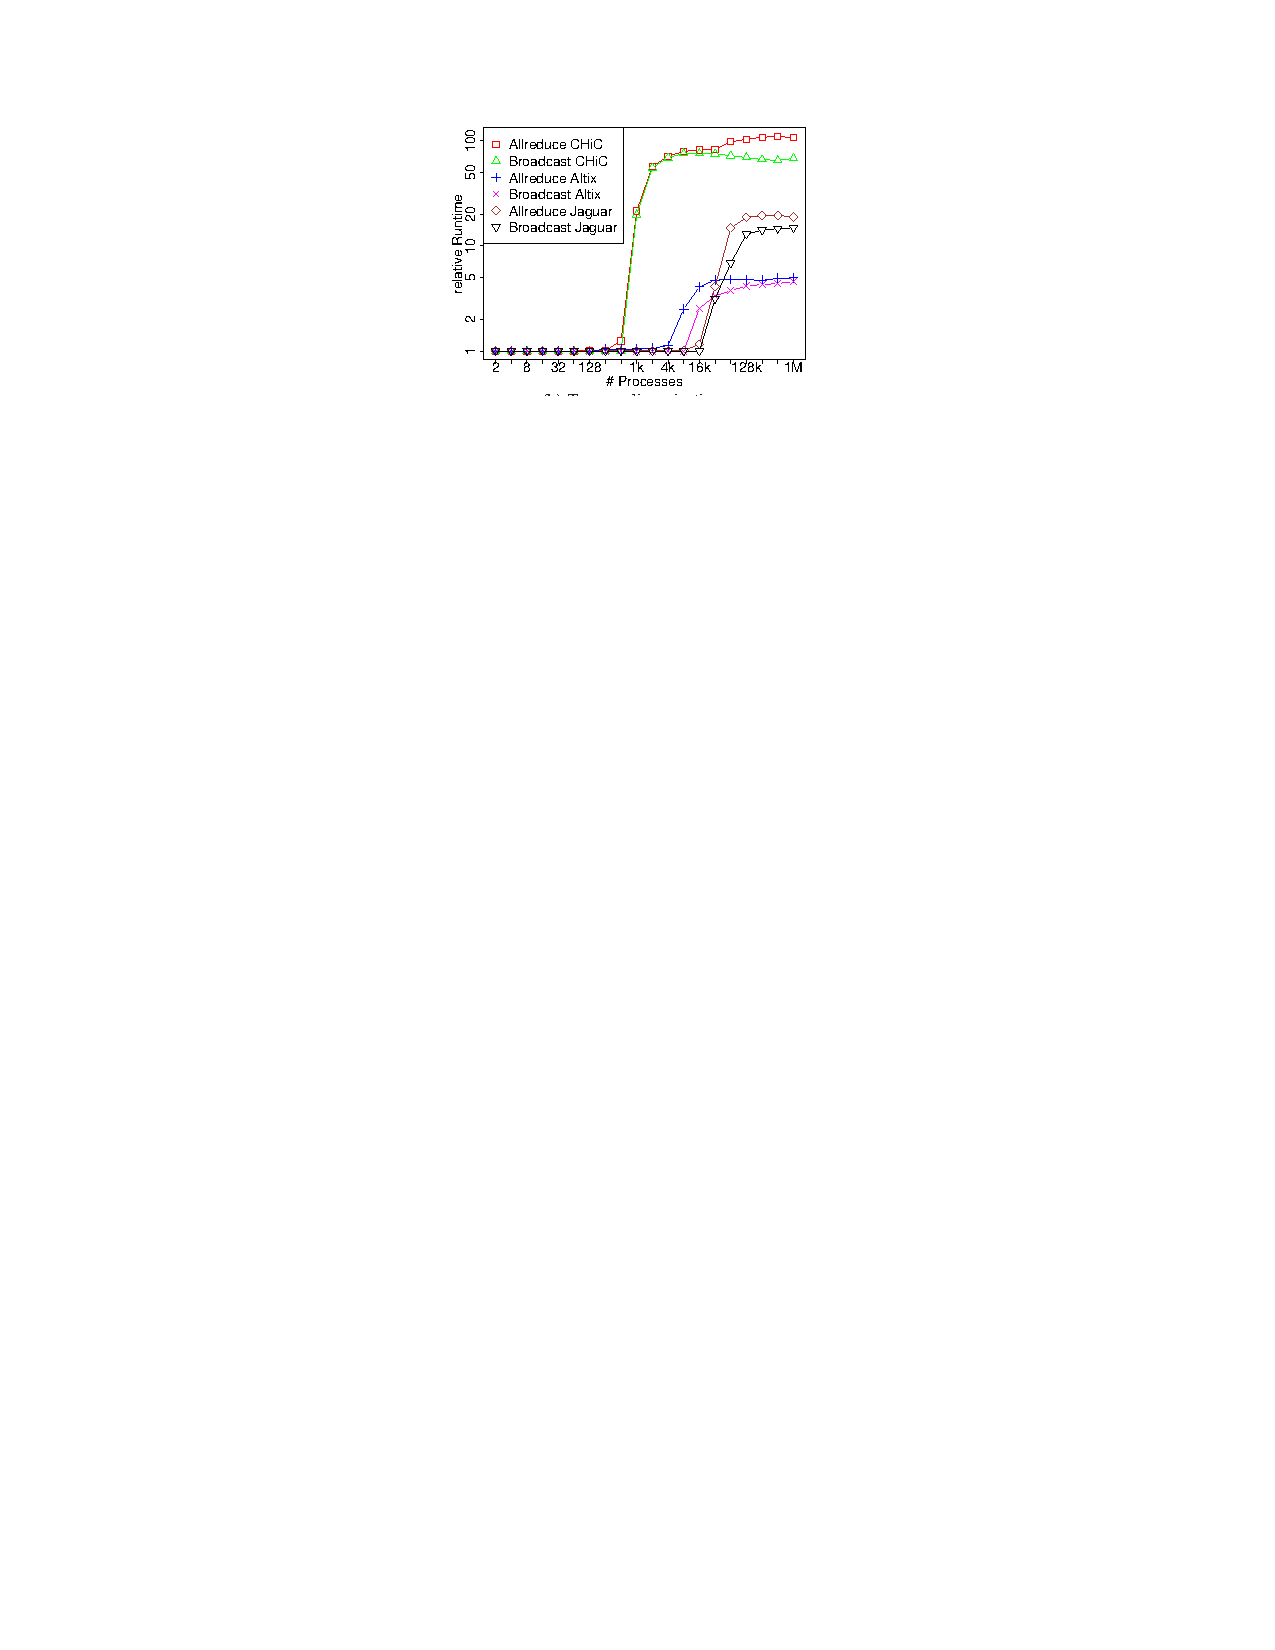
\includegraphics[width=\textwidth]{/Users/kale2/hybridscheduling/images/NoiseAmpProblem-sim}}
\begin{center}
\small Courtesy Hoefler, Lumsdaine, et al
\end{center}
\end{columns}
\end{frame}

\begin{frame}[Noise Amplification Problem for Bulk-synchronous Simulations]
\frametitle{Generalized  Performance Irregularity Amplification Problem}
\begin{columns}
\column{0.5\textwidth}
\begin{enumerate}
\item \tiny Non-deterministic execution within node slows down HPC codes disproportionately at scale.
\item \tiny Because apps are mostly synchronous, noise delays entry into MPI call.
\item \tiny likelihood of imbalance insignificant on single node, but non-negligible at very larger scales
\item \tiny Hybrid MPI+X apps give opportunity because they can allow for moving noise off critical path using X model.
\item \tiny \textit{Problem holds for any uncoordinated localized performance irregularity, and not just OS noise.}
%\item \small \textit{Can consider any multiple-level parallel model where there are multiple levels of parallelism.}
\end{enumerate}
\column{0.5\textwidth}
\framebox{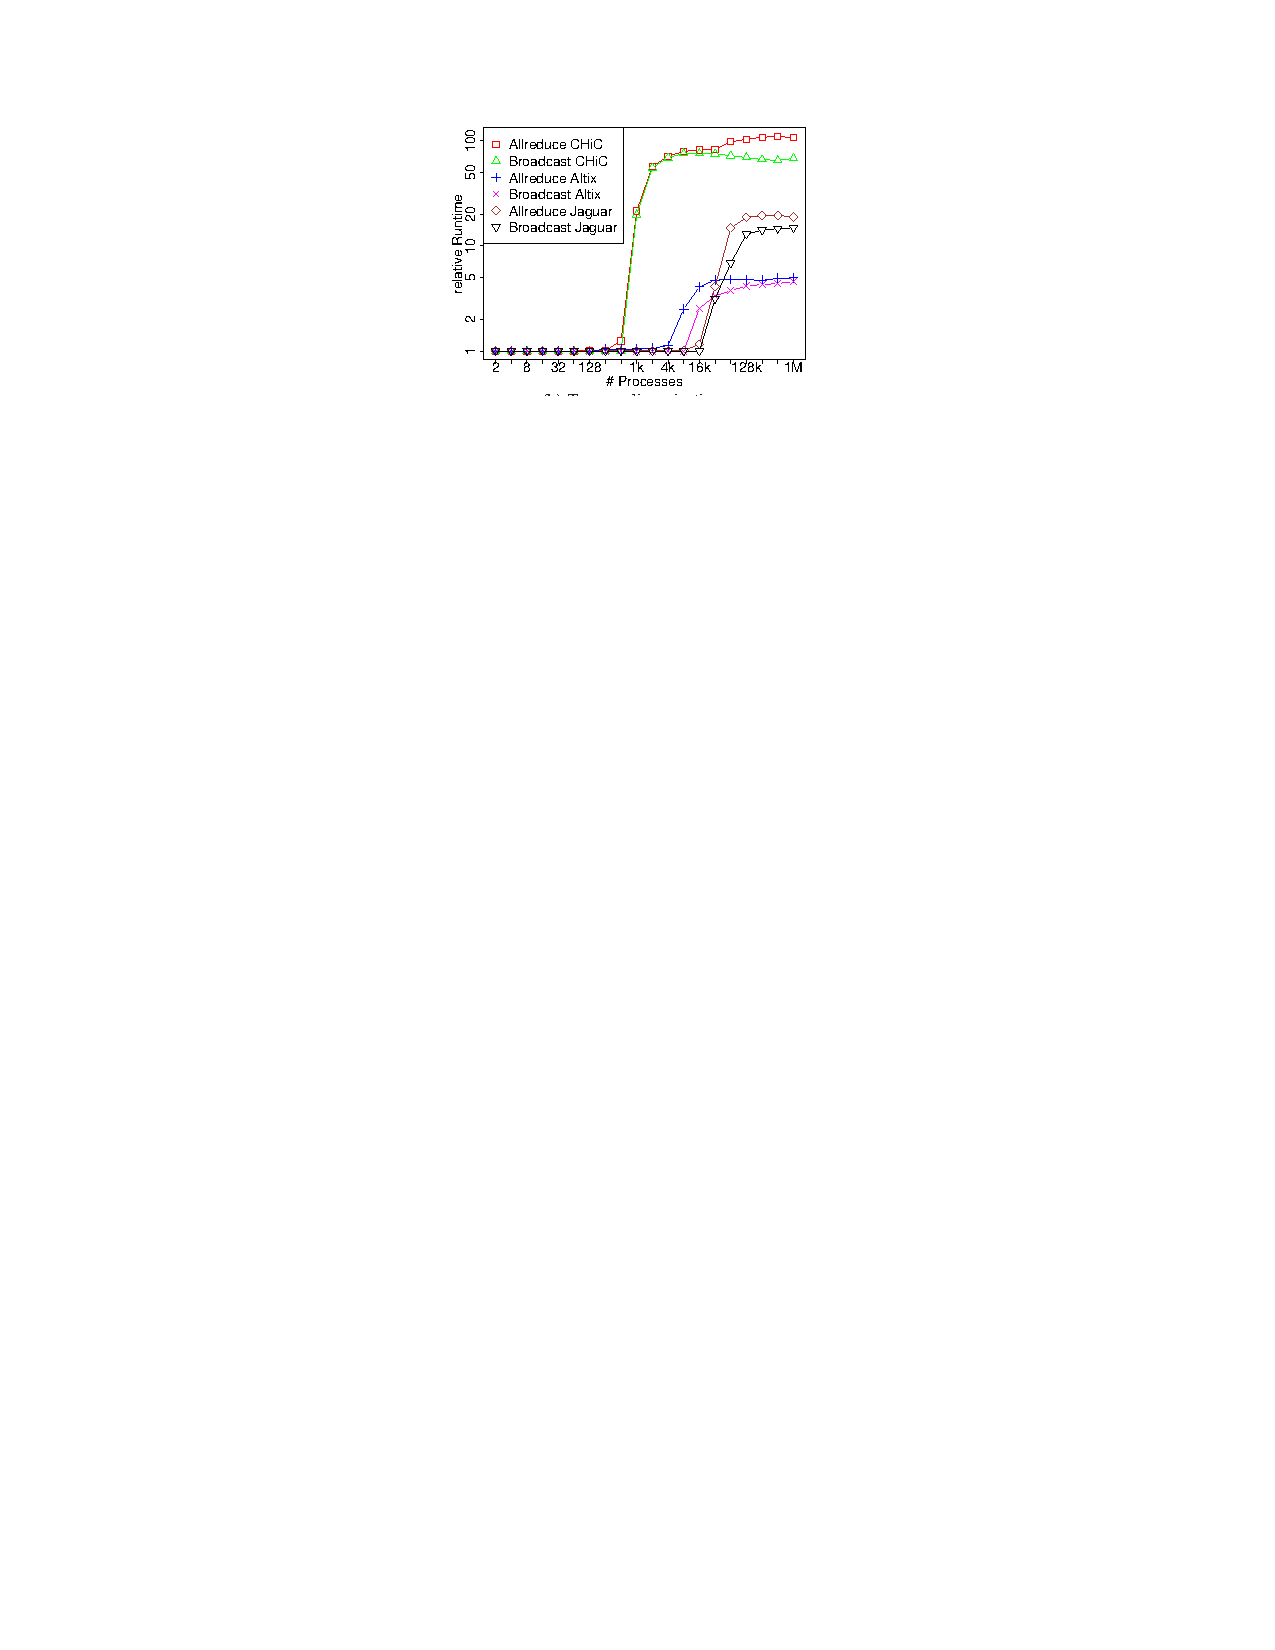
\includegraphics[width=\textwidth]{/Users/kale2/hybridscheduling/images/NoiseAmpProblem-sim}}
\begin{center}
\small Courtesy Hoefler, Lumsdaine, et al
\end{center}
\end{columns}
\end{frame}

\begin{frame}[Noise Amplification Problem for Bulk-synchronous Simulations]
\frametitle{Generalized perf irregularity Amplification Problem}
\begin{columns}
\column{0.5\textwidth}
\begin{enumerate}
\item \tiny Non-deterministic imbalance within node slows down HPC codes disproportionately at scale
\item \tiny Because apps are mostly synchronous, non-deterministic imbalance delays entry into MPI call
\item \tiny Likelihood of imbalance insignificant on single node, but non-negligible at very larger scales
\item \tiny Hybrid MPI+OpenMP apps give opportunity because they can allow for moving noise off critical path using OpenMP model, and they already have a dynamic schedule implemented in runtime.
\item \tiny \textit{Problem holds for any uncoordinated localized performance irregularity, and not just OS noise.}
\end{enumerate}
\column{0.5\textwidth}
\framebox{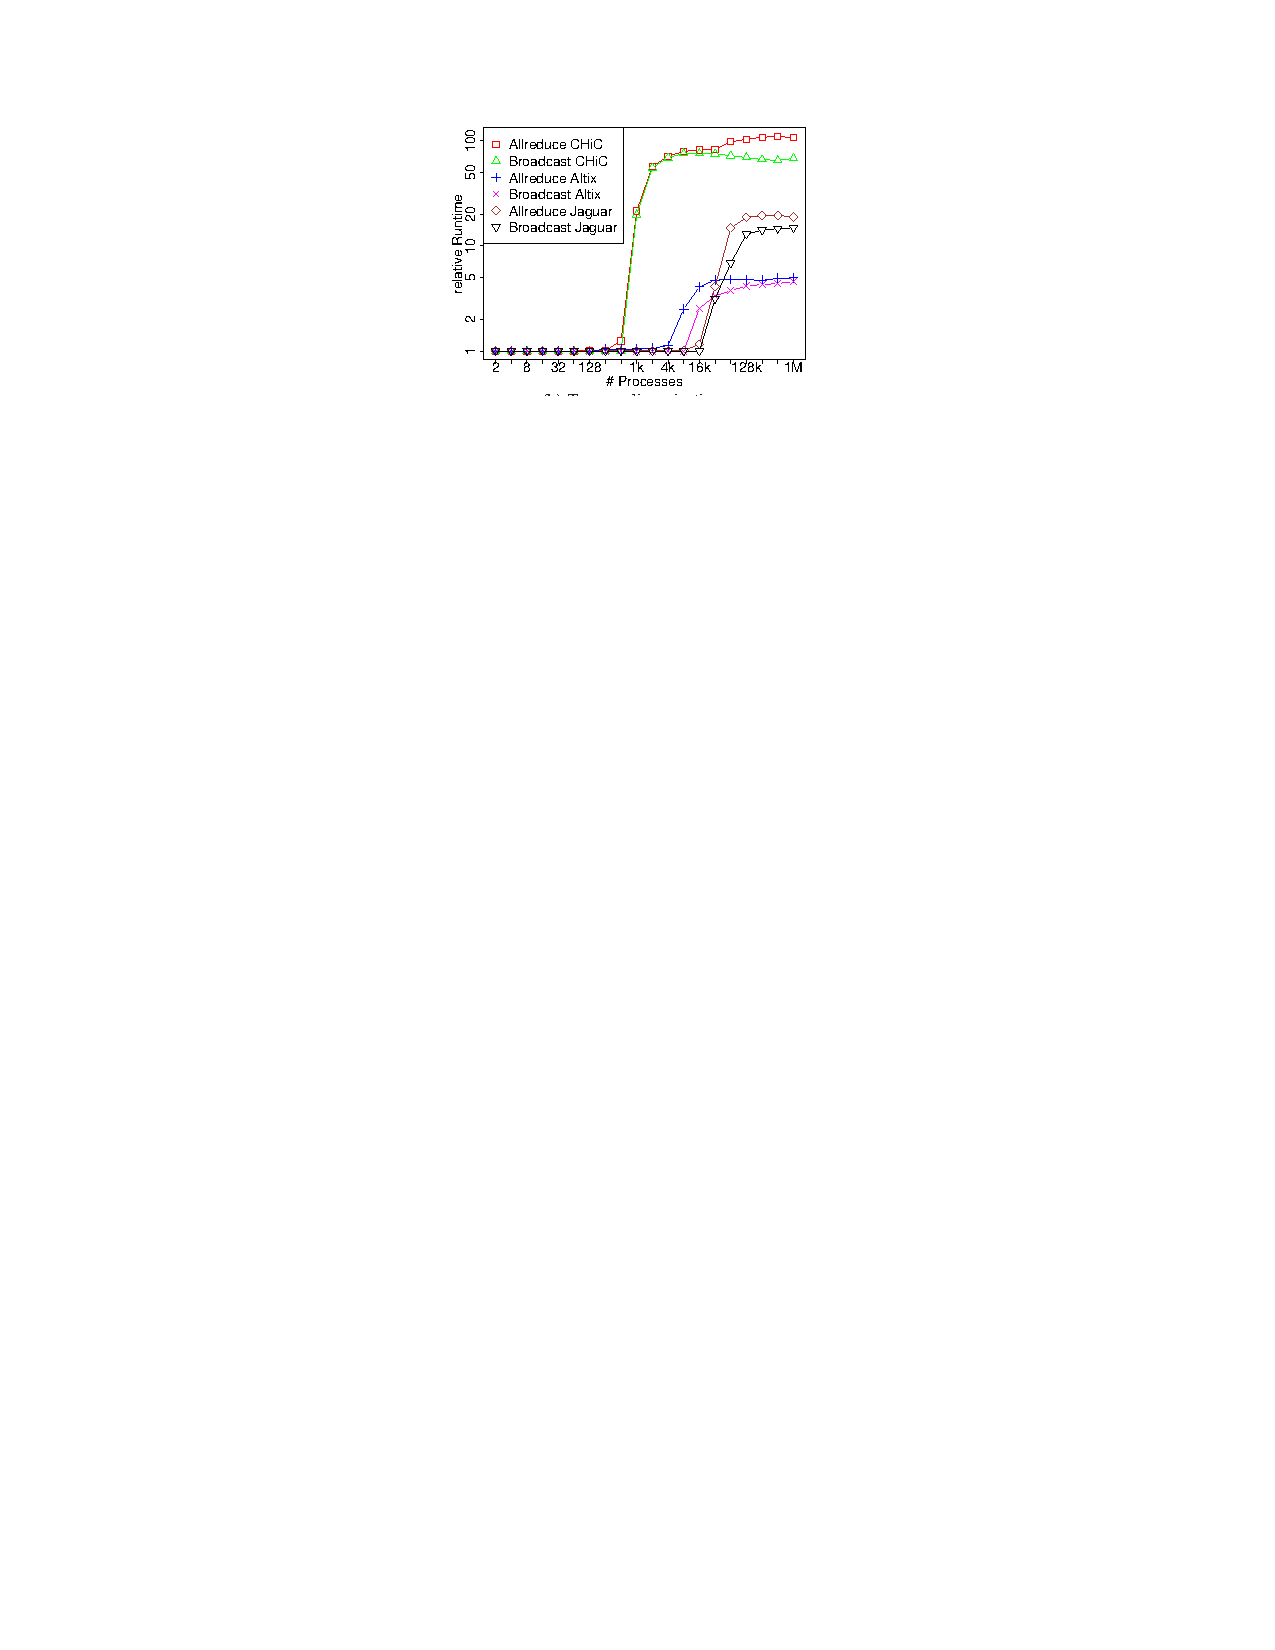
\includegraphics[width=\textwidth]{/Users/kale2/hybridscheduling/images/NoiseAmpProblem-sim}}
\begin{center}
\small Courtesy Hoefler, Lumsdaine, et al
\end{center}
\end{columns}
\end{frame}

\begin{frame}
\frametitle{Model Bulk-synchronous code }
\lstinputlisting{/Users/kale2/hybridscheduling/listings/mpi-bulk-synch.c}
\begin{center}
\includegraphics[scale=0.65]{/Users/kale2/hybridscheduling/images/appTimestep}
\end{center}
\end{frame}

\begin{frame}
\frametitle{Model Bulk-synchronous Hybrid MPI+OpenMP code }
\lstinputlisting{/Users/kale2/hybridscheduling/listings/omp-static.c}
\begin{center}
\includegraphics[scale=0.45]{/Users/kale2/hybridscheduling/images/emptySchedImage}
\end{center}
\end{frame}

\begin{frame}
\frametitle{Model Hybrid MPI+OpenMP Code}
\visible<1->{\lstinputlisting{/Users/kale2/hybridscheduling/listings/omp-static.c}}
\visible<2->{\includegraphics[scale=0.35]{/Users/kale2/hybridscheduling/images/legend-appTimestep}}
\end{frame}

\begin{frame}
\frametitle{Conceptual Diagram of Timestep }
%\lstinputlisting{/Users/kale2/hybridscheduling/listings/omp-static.c}
\includegraphics[scale=0.35]{/Users/kale2/hybridscheduling/images/legend-appTimestep}
\begin{center}
\includegraphics[scale=0.45]{/Users/kale2/hybridscheduling/images/appTimestep}
\end{center}
%\includegraphics[scale=0.35]{/Users/kale2/hybridscheduling/images/legend-twocol}
%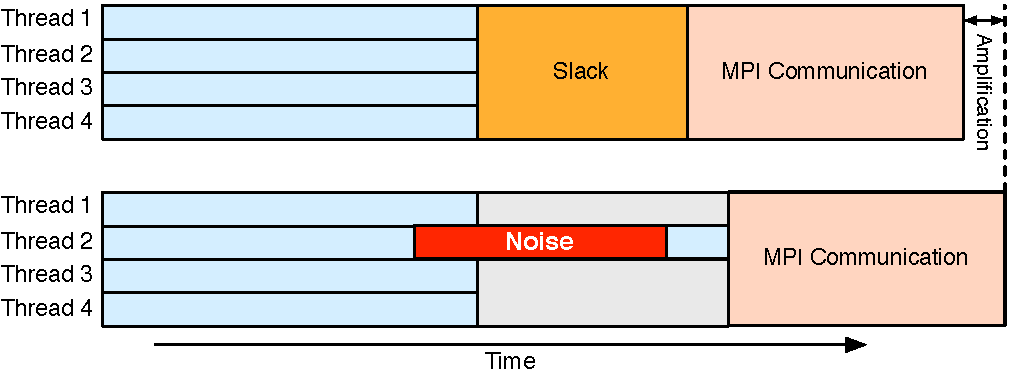
\includegraphics[scale=0.45]{/Users/kale2/hybridscheduling/images/static-schedule}
\begin{center}
\includegraphics[scale=0.45]{/Users/kale2/hybridscheduling/images/emptySchedImage}
\end{center}
\end{frame}

\begin{frame}
\frametitle{Amplification}
\includegraphics[scale=0.35]{/Users/kale2/hybridscheduling/images/legend-static}
\begin{center}
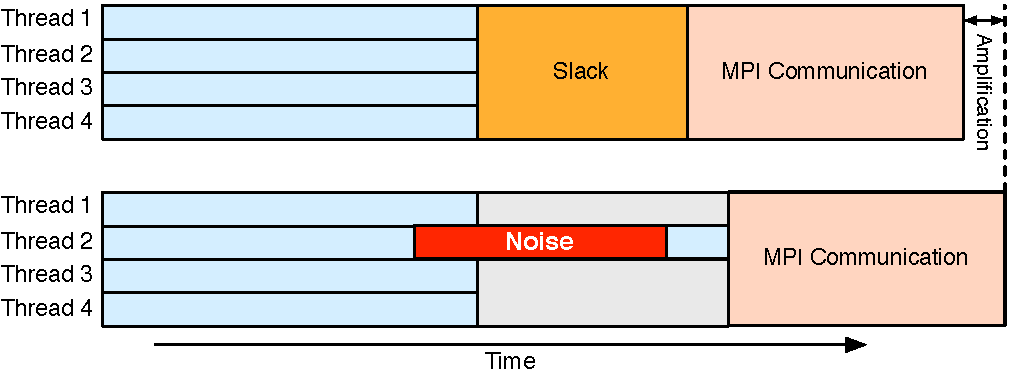
\includegraphics[scale=0.45]{/Users/kale2/hybridscheduling/images/static-schedule}
\end{center}
\begin{center}
\includegraphics[scale=0.45]{/Users/kale2/hybridscheduling/images/emptySchedImage}
\end{center}
\end{frame}


\begin{frame}
\frametitle{Assumption: Application is load balanced }
\begin{itemize}
\item \small Assume that problem is load balanced across MPI processes.
\item \small If problem isn't load balanced across MPI processes, then some other ``classical'' load balancer takes care of it.
\end{itemize}
\end{frame}

%\begin{frame}
%\frametitle{Localized Coordinated+Uncoordinated Load Imbalance}
%\begin{itemize}
%\item \small Assume that problem is load balanced across MPI processes.
%\item \small If problem isn't load balanced across MPI processes, then some other ``classical'' load balancer takes care of it.
%\item \small Imbalance stays within-node, or within racks
%\end{itemize}
%\end{frame}


\begin{frame}
\frametitle{Uncoordinated Transient Load Imbalance}
\begin{itemize}
\item \small If in iteration 304, if node 7 experiences excess work, it is not necessary that other nodes experience excess work in the same iteration.
\item \small If core 3 of node 7 has excess work, it does not mean core 3 of node 19 has excess work.
\item \small No pattern of load imbalances across MPI processes(show across space).
\end{itemize}
\end{frame}

\begin{frame}
\frametitle{Traditional load balancers are of no help }
\begin{enumerate}
\item \small Traditional load balancers,e.g. Measurement-based load balancer, handle load imbalances that persist over time
\item \small Here, no patterns of load imbalance across time, so can't use measurement-based load balancing.
\item \small Load imbalance happens with a certain probability on a node.
\item \small On each timestep, load imbalance happens with higher probability as we scale (as probabilities add up).
\item \small The probability of load imbalance occurring in one timestep increases as we scale (as probabilities add up).
\end{enumerate}
\end{frame}

\begin{frame}
\frametitle{Localized Uncoordinated Transient Load Imbalance}
\begin{itemize}

\end{itemize}
\end{frame}




%1. TO DO: do excel simulation for noise amplification curves for delta, p and T.  Also, consider modified delta after mitigation .

%%2. TO DO :  do experimentation for check asynchronous collectives

%\begin{frame}
%\frametitle{Why not asynchronous collectives?}
%\begin{itemize}
%\item suppose you have fraction f of work(from the next timestep/iteration) that you can do before results of the collective are available . What is the impact on amplification?
%\item
%\end{itemize}
%\end{frame}

\begin{frame}
\frametitle{Localized Uncoordinated Transient Amplifying Load Imbalance}
\begin{itemize}
\item \small If slack, then some local load imbalance can be absorbed.
\item \small If little to no slack, then load imbalance will create load imbalance across processes.
\end{itemize}
\end{frame}

\begin{frame}
\frametitle{Moving work off critical path with Dynamic Scheduling}
\includegraphics[scale=0.35]{/Users/kale2/hybridscheduling/images/legend-dynamic}
\begin{center}
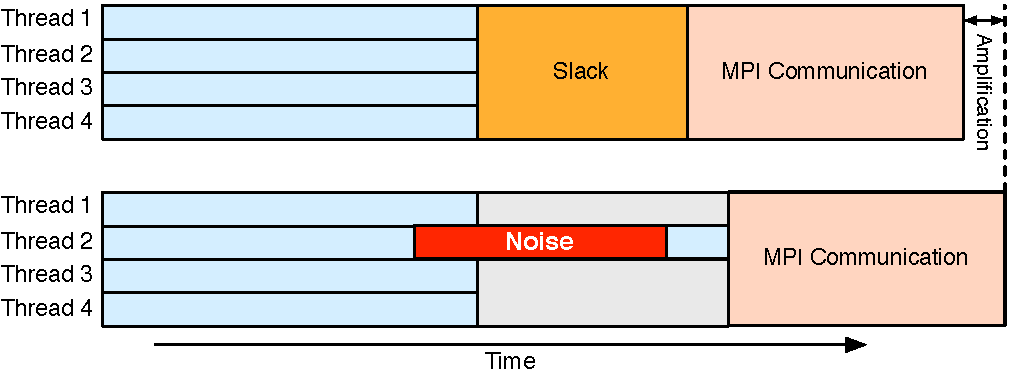
\includegraphics[scale=0.45]{/Users/kale2/hybridscheduling/images/static-schedule}
\end{center}
\begin{center}
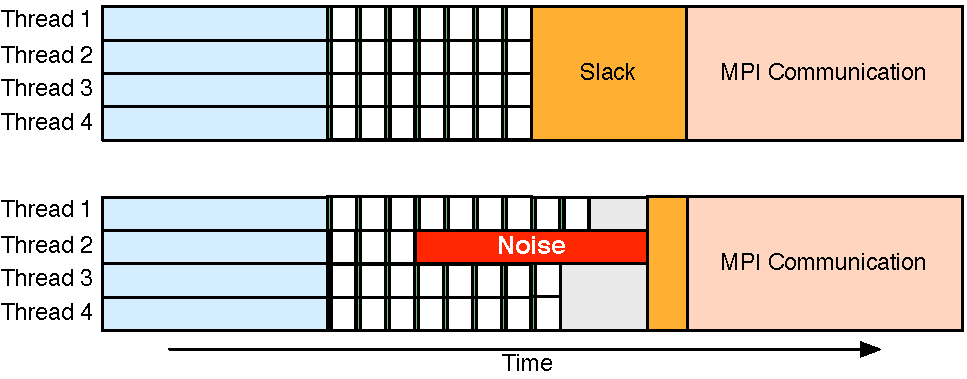
\includegraphics[scale=0.45]{/Users/kale2/hybridscheduling/images/dynamic-schedule}
\end{center}
\end{frame}

\begin{frame}
\frametitle{Resilient Scheduling}
\includegraphics[scale=0.35]{/Users/kale2/hybridscheduling/images/legend-dynamic}
\begin{center}
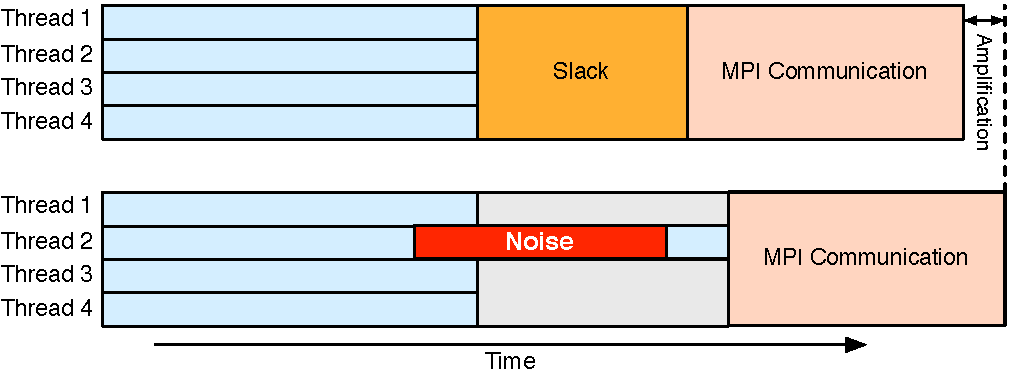
\includegraphics[scale=0.45]{/Users/kale2/hybridscheduling/images/static-schedule}
\end{center}
\begin{center}
\includegraphics[scale=0.45]{/Users/kale2/hybridscheduling/images/hybsched}
\end{center}
\end{frame}

\comments{
\begin{frame}
\frametitle{Model}
\begin{center}
\includegraphics<1>[scale=0.45]{/Users/kale2/hybridscheduling/images/legend-onecol}
\includegraphics<1>[scale=0.45]{/Users/kale2/hybridscheduling/images/appTimestep}
\includegraphics<2>[scale=0.45]{/Users/kale2/hybridscheduling/images/static-schedule}
\includegraphics<2>[scale=0.45]{/Users/kale2/hybridscheduling/images/emptySchedImage}
\end{center}
\end{frame}

\begin{frame}
\frametitle{Resilient Scheduling Strategy applied to MPI+OpenMP code}
\begin{figure}
\includegraphics[scale=0.4]{/Users/kale2/hybridscheduling/images/hybsched}
\end{figure}
\begin{figure}
\includegraphics[scale=0.4]{/Users/kale2/hybridscheduling/images/slackConscious-schedule}
\end{figure}
%\begin{figure}
%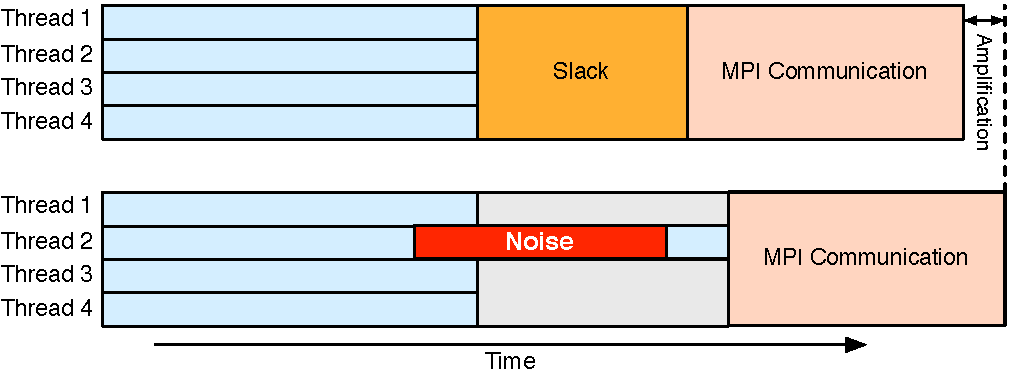
\includegraphics[scale=0.3]{/Users/kale2/hybridscheduling/images/static-schedule}
%\end{figure}
\end{frame}
}

\begin{frame}
\frametitle{ What is the right amount of dynamic scheduling to use?(theory) }
\begin{itemize}
\item theoretical analysis
\end{itemize}
\end{frame}


% add in where ROSE comes in, and source to source comes in.
% put in MPI application specifics and code
% put in impact of compiler (icc vs. gcc)

\begin{frame}
\frametitle{Resilient Scheduling Strategy Applied to Model Synchronous MPI+OpenMP Code}
\lstinputlisting{/Users/kale2/hybridscheduling/listings/omp-static.c}
\lstinputlisting{/Users/kale2/hybridscheduling/listings/omp-hybrid.c}
\end{frame}

\begin{frame}
\frametitle{High-level Software Design}
\includegraphics[width=\textwidth]{/Users/kale2/hybridScheduling/images/architecture}
\end{frame}

\begin{frame}
\frametitle{Scaling with Resilient Scheduling}
\begin{figure}[h]
\label{fig:app-scaling-hera}
\begin{center}
\includegraphics[width=\columnwidth]{/Users/kale2/hybridscheduling/plots/app-scaling-hera}
\end{center}


\begin{center}
\tiny Percent speedup of callsite strategy over baseline stat. sched. on sierra.
\end{center}
\end{figure}

\begin{figure}[h]
\label{fig:app-scaling-rzuseq}
\begin{center}
%\includegraphics[width=\columnwidth]{/Users/kale2/hybridscheduling/plots/app-scaling-rzuseq}
\includegraphics[width=\columnwidth]{plots/app-scaling-rzuseq}

\end{center}
\begin{center}
\tiny Percent speedup of callsite strategy over baseline stat. sched. on rzuseq.
\end{center}
\end{figure}

%\begin{itemize}
%\small \item \tiny \textit{Static-Hybrid} gives moderate perf gains, as can be seen in figure~\ref{fig:app-scaling-hera}.
%\item \tiny Resilient-Callpath gives best perf. gain of all slack-conscious strategies, as seen in figure~\ref{fig:app-scaling-hera}.
%\item \tiny Resilient-Coll and Resilient-Naive give limited perf gains, likely due to
%  mispredictions, which outweigh the overhead of the prediction.
%\item \tiny As seen in figure ~\ref{fig:app-scaling-rzuseq}, the \textit{Resilient-Callpath} method does not cause large degradations, showing
%that using the methodology does not interfere greatly with the performance of the application.
%\end{itemize}
\end{frame}

\begin{frame}
\frametitle{Adaptive MPI Slack Prediction Mechanism Evaluation}
%\begin{columns}
%\column{0.5\textwidth}
\begin{figure}[h]
\begin{center}
\includegraphics[scale=0.47]{/Users/kale2/hybridscheduling/plots/strategy-comp-hera}
\end{center}
%\begin{center}
%{\tiny Percent speedup over stat. sched. for different slack pred. strategies for sierra at largest scale.}
%\end{center}
\end{figure}
\begin{figure}[h]
\label{fig:strategy-comp-useq}
\begin{center}
\includegraphics[scale=0.47]{/Users/kale2/hybridscheduling/plots/strategy-comp-rzuseq}
\end{center}
%\begin{center}
%\tiny Percent speedup over stat. sched. for different slack pred. strategies for rzuseq at largest scale.
%\end{center}
\end{figure}
%\column{0.5\textwidth}
%\end{columns}
\end{frame}

\comments{
\begin{frame}
\frametitle{Adaptive MPI Slack Prediction Mechanism Evaluation}
\begin{columns}
\column{0.5\textwidth}
\begin{figure}[h]
\label{fig:slackOvhd-hera}
\begin{center}
  \small
  \input{/Users/kale2/hybridscheduling/plots/slackOvhd-hera}
\end{center}
\end{figure}


\begin{figure}[h]
\label{fig:slackOvhd-useq}
\begin{center}
  \small
  \input{/Users/kale2/hybridscheduling/plots/slackOvhd-useq}
\end{center}
\end{figure}

\column{0.5\textwidth}
\begin{figure}[h]
\label{fig:slackError-hera}
\begin{center}
  \small
  \input{/Users/kale2/hybridscheduling/plots/slackError-hera}
\end{center}
\end{figure}
\begin{figure}[h]
\label{fig:slackError-useq}
\begin{center}
  \small
  \input{/Users/kale2/hybridscheduling/plots/slackError-useq}
\end{center}
\end{figure}
\end{columns}
\end{frame}

}

%\begin{frame}
%\frametitle{Variants of  $\mu$-Scheduling}
%\begin{itemize}
%\item \small Can categorize scheduling strategies based on compile-time, runtime, across MPI regions, and across application runs.
%\item \small Locality-conscious scheduling (runtime + across timesteps)
%\item \small Variable Tasklet Granularity $\mu$-scheduling(Compile time + runtime): Resilient to variable length noise.
%\item \small N-stage scheduling(compiletime + runtime)
%\item \small Weighted Dynamic $\mu$-scheduling: Resilient to periodic noise (runtime + across timesteps)
%\item \small Risk Analysis of slack-conscious scheduling (across timesteps)
%\item \small Machine learning of slack patterns to adjust Resilient-Collectives (Across runs)
%\end{itemize}
%\end{frame}


\begin{frame} [Handling Semi-persistent load imbalances]
\frametitle{Localized Uncoordinated Semi-Transient/Semi-Persistent Load Imbalance}
\begin{itemize}
\item \small No patterns of load imbalance across time, so can't use measurement-based load balancing.
\item \small Load imbalance happens with a certain probability on a node.
\item \small On each timestep, load imbalance happens with more frequency as we scale(as probabilities add up).
\end{itemize}
\end{frame}


\begin{frame} [Handling Semi-persistent load imbalances(Solution) ]
\frametitle{Localized Uncoordinated Semi-Transient/Semi-Persistent Load Imbalance}
\begin{itemize}
\item \small No patterns of load imbalance across time, so can't use measurement-based load balancing.
\item \small Load imbalance happens with a certain probability on a node.
\item \small On each timestep, load imbalance happens with more frequency as we scale(as probabilities add up).
\end{itemize}
\end{frame}

\begin{frame} [Handling Variable length excess work  ]
\frametitle{Localized Uncoordinated Semi-Transient/Semi-Persistent Load Imbalance}
\begin{itemize}
\item \small No patterns of load imbalance across time, so can't use measurement-based load balancing.
\item \small Load imbalance happens with a certain probability on a node.
\item \small On each timestep, load imbalance happens with more frequency as we scale(as probabilities add up).
\end{itemize}
\end{frame}


\begin{frame} [Handling Variable length excess work (Solution)  ]
\frametitle{Localized Uncoordinated Semi-Transient/Semi-Persistent Load Imbalance}
\begin{itemize}
\item \small No patterns of load imbalance across time, so can't use measurement-based load balancing.
\item \small Load imbalance happens with a certain probability on a node.
\item \small On each timestep, load imbalance happens with more frequency as we scale(as probabilities add up).
\end{itemize}
\end{frame}


\begin{frame} [Add'l note: Reducing the cost of scheduling in the dynamic region ]
\frametitle{Reducing cost of sched}
\begin{itemize}
\item \small -
\item \small -
\end{itemize}
\end{frame}

\begin{frame} [Reducing the cost of scheduling in the dynamic region ]
\frametitle{Reducing cost of sched(solution)}
\begin{itemize}
\item \small -
\item \small -
\end{itemize}
\end{frame}


\begin{frame} [Tunable locality-aware scheduling]
\frametitle{Alternate solution: Tunable locality-aware scheduling}
\begin{itemize}
\item \small -
\item \small need to tune scheduler, still fits theme of our scheduler
\end{itemize}
\end{frame}


\begin{frame}
\frametitle{Advanced problem: u.l.t load imbalance across MPI processes on the same node(or across processes on different nodes, nearby to each other) }
\begin{itemize}
\item \small -
\item \small -
\end{itemize}
\end{frame}

\begin{frame}
\frametitle{Advanced solution: Stealing work across MPI processes/nodes that are local to each other}
\begin{itemize}
\item \small -
\item \small use MPI rma
\end{itemize}
\end{frame}



\begin{frame}
\frametitle{ Dealing with multi-core interconnect and mem hierarchy}
\begin{itemize}
\item \small
\item \small need to tune scheduler, still fits theme of our scheduler
\end{itemize}
\end{frame}

\begin{frame}
\frametitle{ Advanced Solution: Use N-stage scheduling}
\begin{itemize}
\item \small -
\item \small need to tune scheduler, still fits theme of our scheduler
\end{itemize}
\end{frame}


\begin{frame}[slack error]
\frametitle{ Problem: dealing with slack misprediction  }
\begin{itemize}
\item \small -
\item \small -
\end{itemize}
\end{frame}

\begin{frame}[slack error]
\frametitle{Advanced Solution: Use risk model }
\begin{itemize}
\item \small -
\item \small -
\end{itemize}
\end{frame}

\begin{frame}
  \frametitle{Conclusions}
  \begin{itemize}
  \item \small Noise difficult to handle through conventional techniques due to complex chain of dependences in MPI collectives.
  \item \small OpenMP provides a way to cost efficiently handle the load imbalance induced by noise.
  \item \small If slowdowns due to noise are small, our runtime does not induce overheads.
  \item \small Feasible to integrate into applications through compiler and adaptive runtime.
  \item \small Can further refine accuracy of slack prediction through risk model.
  \item \small Plan to provide more loosely coupled interface between OpenMP and MPI, or between any two programming models.
  \end{itemize}
\end{frame}
